\documentclass[11pt]{article}
\usepackage{amsmath,amssymb,booktabs,graphicx,xcolor,hyperref}
\usepackage[margin=1in]{geometry}
\definecolor{ink}{RGB}{26,64,76}
\hypersetup{colorlinks=true,urlcolor=ink,linkcolor=ink,citecolor=ink,pdftitle={Fully symmetric no-three-in-line sets and an obstruction at order 47}}
\newcommand{\lastorder}{65}
\newcommand{\D}{D_4}
\newcommand{\F}{F}
\newcommand{\Ocal}{\mathcal O}
\title{Fully symmetric no-three-in-line sets and an obstruction at order 47}
\author{} % Human authors: add names after verifying the computation and priority.
\date{Research draft, 19 November 2026}
\begin{document}
\maketitle
\begin{abstract}
Let $F(n)$ be the largest size of a no-three-in-line set on an $n\times n$ integer grid that is invariant under all eight symmetries of the square. We compute $F(n)$ and the number of maximizers for every odd $3\le n\le\lastorder$. This extends the odd-order portion of Flammenkamp's public minimal-defect table, which gives maxima through $n=39$. At $n=47$ a unique $92$-point set attains the odd-order symmetry bound $2n-2$. At $n=61$ the defect $2n-F(n)$ first reaches $10$ on an odd board; there are $295$ maximizers. The computation represents a configuration by disjoint pairs and singletons of positive coordinate magnitudes. We also prove that a fully symmetric set attaining $2n-2$ either admits no further grid point, even without imposing symmetry, or has exactly two completions of size $2n$. For the unrestricted problem we show that every $94$-point configuration on the $47$-board contains at most $68$ points forming a fully symmetric subset. Equivalently, restoring full symmetry by deletion costs at least $26$ points. Counts, coordinates and code are supplied.
\end{abstract}

\section{The result and its scope}
The ordinary no-three-in-line problem asks for the largest subset of an $n\times n$ grid with no three points on any one Euclidean line. Its row bound is $2n$. Imposing symmetry has helped find many examples attaining that bound \cite{flam92,flam98,prell}. Here symmetry is a \emph{condition on the final set}, not just a search heuristic. We impose the full dihedral group $\D$ of order eight. In particular, our upper bounds are \emph{not} upper bounds for the unrestricted problem.

Write $n=2m+1$ and centre the board at the origin, so its coordinates lie in $[-m,m]^2\cap\mathbb Z^2$. Let $C(n)$ be the number of sets attaining $F(n)$. Each such set is fixed by every symmetry of the board, so counting labelled subsets or counting modulo $\D$ gives exactly the same number. Translations are not an additional equivalence. An optimum is a largest set; a maximal set need only be incapable of single-point extension.

\textbf{Computational result.} Table~\ref{tab:results} gives $F(n)$ and $C(n)$ for odd $35\le n\le\lastorder$. In the entire odd range $3\le n\le\lastorder$, the sizes attaining the bound $2n-2$ are precisely
\[
3,5,7,9,11,13,15,17,25,33,47.
\]
At these orders the total number of ceiling-attaining configurations is $24$. Of these, only the axial cross on the $3\times3$ board can be enlarged by even one point. A separate consequence for unrestricted optima is given in Section~\ref{sec:core}.

The comparison is with the \texttt{full} column of the public minimal-defect table dated 3 May 2026 \cite{defects}, not with the separate catalogue of configurations of size $2n$ \cite{catalogue}. The former gives defects but not multiplicities at $35,37,39$; the subsequent odd-order \texttt{full} entries are blank in that snapshot. A blank is not a zero or proof of publication priority.

\begin{table}[ht]
\centering
\begin{tabular}{r r r r r}
\toprule
$n$ & $F(n)$ & $2n-F(n)$ & unused magnitudes & $C(n)$\\
\midrule
% BEGIN DATA
35 & 64 & 6 & 1 & 17 \\
37 & 68 & 6 & 1 & 5 \\
39 & 72 & 6 & 1 & 17 \\
41 & 76 & 6 & 1 & 3 \\
43 & 80 & 6 & 1 & 12 \\
45 & 84 & 6 & 1 & 3 \\
47 & 92 & 2 & 0 & 1 \\
49 & 92 & 6 & 1 & 4 \\
51 & 96 & 6 & 1 & 6 \\
53 & 100 & 6 & 1 & 1 \\
55 & 104 & 6 & 1 & 2 \\
57 & 108 & 6 & 1 & 1 \\
59 & 112 & 6 & 1 & 5 \\
61 & 112 & 10 & 2 & 295 \\
63 & 116 & 10 & 2 & 60 \\
65 & 120 & 10 & 2 & 177 \\
% END DATA
\bottomrule
\end{tabular}
\caption{Maxima and counts under full square symmetry. The machine-readable table also includes every odd order from 3 to 33. A drop in $F(n)/(2n)$ need not mean a drop in $F(n)$ itself: for example $F(59)=F(61)=112$.}\label{tab:results}
\end{table}

\section{Magnitudes, orbits and defects}
For $0\le a\le b\le m$, let $\Ocal(a,b)$ be the orbit of $(a,b)$ under sign changes and coordinate interchange. The centre cannot coexist with any other orbit: it is the midpoint of two opposite points. A generic orbit $0<a<b$ has eight points. The axial orbit $\Ocal(0,b)$ and the diagonal orbit $\Ocal(b,b)$ each have four. Every individual orbit lies on a circle and hence contains no collinear triple.

\textbf{Lemma 1 (disjoint magnitudes).} \emph{In a nontrivial admissible union of orbits, a positive coordinate magnitude appears in at most one orbit. If $k$ of the $m$ positive magnitudes are unused, the union has exactly $4(m-k)$ points.}

\emph{Proof.} Fix a magnitude $r>0$. A generic or diagonal orbit using $r$ contributes two points in the row $y=r$. An axial orbit using $r$ contributes the single point $(0,r)$ there; there is only one such orbit. Thus two distinct orbits using $r$ put at least three different points in that row. A generic orbit uses two magnitudes and contributes eight points; each exceptional orbit uses one and contributes four. Summing proves the formula.\hfill$\square$

Disjointness is necessary, not sufficient: lines of other slopes still matter. We can now regard an orbit union as a partial matching of $\{1,\dots,m\}$, with unused vertices and two possible types of singleton (axis or diagonal). Two axial singletons are incompatible on an axis, and two diagonal singletons on a long diagonal. Lemma~1 gives
\[
F(2m+1)\le 4m=2n-2,\qquad 2n-F(n)=2+4k
\]
where $k$ is the smallest feasible number of omissions. The possible defect levels are therefore $2,6,10,\ldots$, not all even integers.

\section{Completion without symmetry}
\textbf{Proposition 2.} \emph{Suppose that a fully symmetric no-three-in-line set $S$ on an odd board, $n\ge3$, has $2n-2$ points. It is either inclusion-maximal among all no-three-in-line sets on that board, or else exactly four individual points can be added and there are exactly two distinct $2n$-point supersets. In the latter case both completions preserve the two diagonal reflections.}

\emph{Proof.} Every positive magnitude is used. If there is no axial orbit, every noncentral row and column is full. Their only possible complement intersection is the centre, which is blocked by any opposite pair. Otherwise let $\Ocal(0,a)$ be the unique axial orbit. The central row and column are full. The only deficient rows and columns have indices $\pm a$, contributing one occupied site each. Consequently the only possible insertions are the four sites $(\pm a,\pm a)$. Symmetry makes them either all individually admissible or all inadmissible. If one is admissible, the two long diagonals of $S$ are empty: any occupied point on either has its opposite on that diagonal and the other diagonal is its rotated image. Two opposite candidate points may therefore be added together. All triples with just one new point were already excluded; the common line of the two new points is an empty diagonal. The two opposite pairs give the two completions. Adjacent pairs overfill a row or column.\hfill$\square$

In the extendible case the $m-1$ nonaxial magnitudes are paired, so $n\equiv3\pmod4$. The two completions are equivalent by a quarter-turn.

\textbf{The $47$-board.} A compact witness for the unique maximizer is the union of the orbits with representatives
\begin{align*}
 &(0,7),(1,11),(2,18),(3,21),(4,19),(5,9),\\[-2pt]
 &(6,23),(8,14),(10,15),(12,20),(13,22),(16,17).
\end{align*}
They use all 23 magnitudes and give $4+11\cdot8=92$ points. Since $(7,7)$ is the midpoint of the selected sites $(5,9)$ and $(9,5)$, Proposition~2 rules out every insertion. Other configurations attain the unrestricted maximum of $94$ \cite{catalogue,prell}.

\begin{figure}[!htb]
\centering
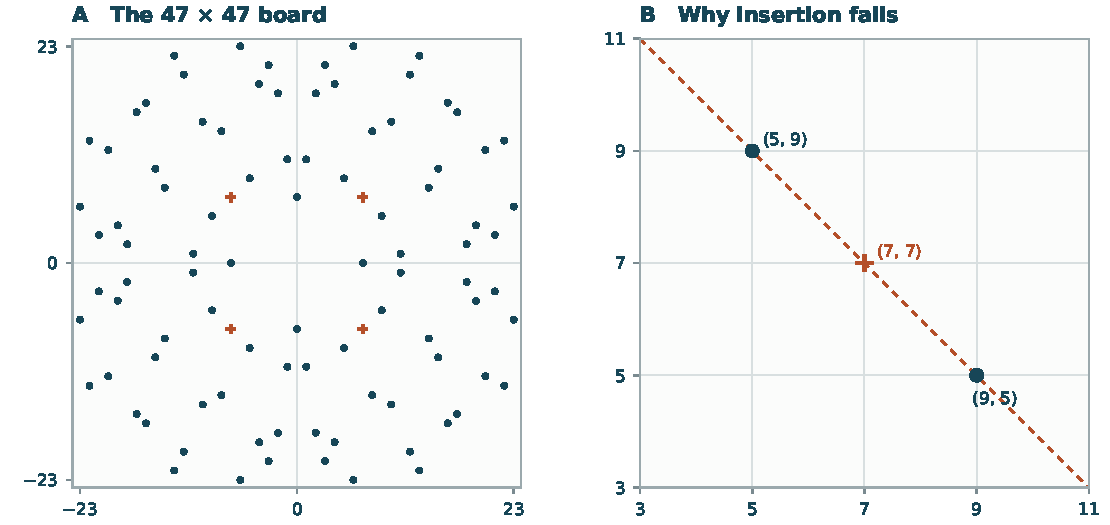
\includegraphics[width=.83\linewidth]{witness47.pdf}
\caption{The $92$-point optimum (left). At right, $(5,9)$ and $(9,5)$ block $(7,7)$. Symmetry rules out the other three marked sites.}\label{fig:47}
\end{figure}

\clearpage
\section{An obstruction for unrestricted solutions at order 47}\label{sec:core}
For an arbitrary set $T$ on the board put $K(T)=\bigcap_{g\in\D}gT$. This is the largest fully symmetric subset of $T$: every invariant subset is contained in the intersection, and the intersection itself is invariant. Flammenkamp, crediting Selfridge, discusses near-symmetry in terms of points missed by an individual isometry and singles out the order-three example \cite{miss}. Here the deletion cost $|T|-|K(T)|$ is with respect to the entire group, with the original board centre fixed.

\textbf{Computational theorem 3.} \emph{If $T$ is any $94$-point no-three-in-line set on the $47\times47$ board, then $|K(T)|\le68$. In particular, at least $26$ points must be removed to leave a fully symmetric set.} This is an upper bound on the core; it does not assert that $68$ is attainable. The input need not belong to any catalogue.

\emph{Exhaustive argument.} Lemma~1 leaves six possible core sizes above $68$, listed below. Enumerate every valid fully symmetric set $S$ at these six sizes. Any $94$-point superset must have two points in every row and column. For each deficient row, count the unoccupied cells that are also in deficient columns and that can be added individually to $S$ without creating a collinear triple. If a row with $r$ old points has fewer than $2-r$ such cells, reject $S$; likewise for columns. This test is necessary and does not assume that the additions are symmetric.

\begin{center}
\begin{tabular}{r r r r}
\toprule
$|S|$ & All symmetric $S$ & Pass row/column test & $94$-point extensions\\
\midrule
92 & 1 & 0 & 0\\
88 & 8 & 0 & 0\\
84 & 278 & 0 & 0\\
80 & 35\,018 & 0 & 0\\
76 & 345\,615 & 2 & 0\\
72 & 10\,536\,015 & 22 & 0\\
\bottomrule
\end{tabular}
\end{center}

Two traversals give the same $10\,916\,935$ sets in total and agree on the actual list of $24$ survivors. The first tests individual cells using the directions to points of $S$; the second precomputes, for each candidate orbit, which pairs of old orbit labels block its representative. For every survivor we then branch over all ways to fill the deficient rows, never exceeding two points in a column and testing new triples by integer determinants. This last stage visits just $18+92=110$ row-search nodes and yields no completion. Since $K(T)$ would itself have appeared in a tested tier, the bound follows.\hfill$\square$

\section{Exhaustion and independent checks}
For a given $k$, the main counter asks for \emph{exactly} $m-k$ used magnitudes. Its input is just $n$: it does not use earlier solutions or catalogue entries. Conflicts arise in two ways. A line through two points of one orbit blocks a second orbit if it meets that orbit. A line through points of two distinct chosen orbits blocks a third orbit that it meets. These tests are exhaustive because a single orbit is automatically admissible and any forbidden triple uses either two or three orbit labels. For each pair of grid points the program walks the integer line in both directions using the difference vector divided by the gcd of its coordinates. In building a conflict list one endpoint may be fixed to its orbit representative: a square symmetry takes any proposed endpoint there while preserving every orbit as a set.

The search maintains the available orbits, the unassigned magnitudes and the remaining omission budget. Choose an unassigned magnitude with the fewest available incident orbits. Branch on selecting each such orbit, plus an omission branch when budget permits. Selection removes all overlapping orbits and all newly incompatible orbits. A magnitude with no options must be omitted; if too many are forced, the branch closes. When the number of unassigned magnitudes equals the remaining omission budget, the current selection is one completion. These branches partition the possible completions according to the unique fate of the chosen magnitude, giving both exhaustiveness and non-duplication by induction. The first nonempty tier gives $F(n)$ and $C(n)$. No optimizer cutoff, sampling assumption or floating-point tolerance enters the result.

The independent counter builds conflicts differently. It enumerates maximal lattice lines of length at least three on the whole grid, labels each cell by its sorted absolute coordinates, and converts triples of cells on a line into two- or three-label exclusions. It keeps partner choices per magnitude, not the first program's bitsets of candidate orbits. A third, short program expands the positive witnesses to ordinary integer coordinates and checks the determinant of \emph{every} point triple. That last check establishes feasibility only; the exhaustive traversals are what give upper bounds and multiplicities. For the main census the two programs agree on all 56 tested tiers of the 32 boards. They visit $5.36$ and $6.44$ billion search nodes respectively. The supplement reports the two counts and node totals at each tier. As a regression test, our maxima agree with all odd-order \texttt{full} entries through 39 and our counts agree wherever those entries give counts.

\paragraph{Scope.} These finite computations do not establish an asymptotic trend and do not settle an open unrestricted order. In particular, the assertion that $61$ is the first odd board with defect ten is a statement about $F$, not about the ordinary maximum. The data expose a nonmonotone deficit: at order 47 it drops back from six to two before rising again.

\appendix
\section{Extensions at unrestricted orders}
The completion question also makes sense without requiring any symmetry of the final set. The October 2026 catalogue supplies two $148$-point seeds of order $74$, two $152$-point seeds of order $76$, and one $156$-point seed of order $78$ \cite{catalogue}. Take one such set $S$ of order $m$ and embed it, without changing distances, in a corner of the $(m+1)$-board. For each of the five sets we found
\[
 |T|\ge 2m+1\ \Longrightarrow\ |S\setminus T|\ge 11
\]
for every no-three-in-line set $T$ on the larger board. This says that one cannot gain even one point while discarding at most ten original ones. It does not rule out any of the target cardinalities on the unrestricted board. The four corner choices are equivalent for these quarter-turn-invariant seeds.

For this finite check, retain the surviving seed points and commit new points one at a time. With a target of $2n-1$ on the $n=m+1$ board, at most one unit of row deficiency may remain. Hence a row deficient by two, or at least one of any two deficient rows, must receive a new point. This also holds for columns. Branch over possible additions on one such line or pair of lines. If $q$ is a trial addition, every surviving seed pair collinear with $q$ forces one of its endpoints to be deleted. Pairs on distinct lines through $q$ are disjoint. A line through $q$ and an earlier addition forces all old points on that line to be deleted; two earlier additions collinear with $q$ forbid it. These are all the new triples. If $T$ exists, at least one branch repeatedly chooses a point in $T$ and deletes only seed points outside $T$. Such a branch cannot exhaust the budget prematurely when $|S\setminus T|\le10$. The five traversals returned zero hits; the exact inputs, node counts and separate search program are supplied in \texttt{extras/}. This auxiliary test was run with one exhaustive implementation.

Separately, the supplement gives thirteen ordinary $2n$-point solutions not contained, under any square isometry, in the same catalogue snapshot. Twelve are asymmetric, including a $112$-point example at order $56$; the remaining one has exact half-turn symmetry at order $36$. These are additional configurations at solved orders, not point-count improvements. Each is given by explicit coordinates and by a reproducible change to a credited catalogue seed. For example, the order-$56$ configuration results from cyclically moving one boundary row of a quarter-turn-invariant seed to the opposite boundary. Such a move preserves the row and column counts but need not preserve Euclidean noncollinearity; we verified the latter on the resulting points, not on a torus.

\paragraph{Reproducibility note.} The accompanying source package contains the C++17 counters, Python verification scripts, input snapshots or checksums, and command lines for the reported calculations. This draft and the accompanying software were developed with AI assistance.

\begin{thebibliography}{9}\small
\bibitem{flam92} A. Flammenkamp, Progress in the no-three-in-line problem, \emph{J. Combin. Theory Ser. A} \textbf{60} (1992), 305--311. \href{https://doi.org/10.1016/0097-3165(92)90012-J}{doi:10.1016/0097-3165(92)90012-J}.
\bibitem{flam98} A. Flammenkamp, Progress in the no-three-in-line problem, II, \emph{J. Combin. Theory Ser. A} \textbf{81} (1998), 108--113. \href{https://doi.org/10.1006/jcta.1997.2829}{doi:10.1006/jcta.1997.2829}.
\bibitem{defects} A. Flammenkamp, Minimal defect for fixed symmetry and grid size, table dated 3 May 2026, \url{https://wwwhomes.uni-bielefeld.de/achim/no3in/table_min_defect}.
\bibitem{catalogue} A. Flammenkamp, The No-Three-in-Line Problem, record log and downloadable configurations, update of 28 October 2026, \url{https://wwwhomes.uni-bielefeld.de/achim/no3in/readme.html}.
\bibitem{miss} A. Flammenkamp, Symmetries in no-three-in-line configurations, section on near symmetry misses, \url{https://wwwhomes.uni-bielefeld.de/achim/no3in/symmetry_remarks.html}.
\bibitem{prell} T. Prellberg, Constraint satisfaction programming for the no-three-in-line problem, \href{https://arxiv.org/abs/2602.07751}{arXiv:2602.07751} (2026), \href{https://doi.org/10.1016/j.jcta.2026.106244}{doi:10.1016/j.jcta.2026.106244}.
\end{thebibliography}
\end{document}
